\documentclass{beamer}
\usetheme{}
\usecolortheme{dolphin}           
\useinnertheme{circles}
\setbeamertemplate{itemize items}[default]
\setbeamertemplate{enumerate items}[default]
\usepackage[T1]{fontenc}
\usepackage[utf8]{inputenc}
\usepackage{lmodern}
\usepackage{amsmath}
\usepackage{booktabs} 
\usepackage{graphicx}        
\usepackage{array}
\usepackage{color}
\makeatletter
\def\zapcolorreset{\let\reset@color\relax\ignorespaces}
\def\colorrows#1{\noalign{\aftergroup\zapcolorreset#1}\ignorespaces}
\makeatother
\setbeamertemplate{navigation symbols}{}
\setbeamertemplate{footline}[frame number]

%--------------------------------------
\title{Monetary and fiscal policy within the EU}
\author{School of Economics, University College Dublin}
\date{Spring 2018}
\begin{document}

%--------------------------------------
\begin{frame}
 \titlepage
\end{frame}
%--------------------------------------

%--------------------------------------
\begin{frame}
  \textbf{Economic Monetary Union}\\
  Established by 1992 Maastricht Treaty
  \begin{itemize}
    \item Decision to form EMU was taken in 1988
  \end{itemize}
  \medskip
  Part of three stage process for euro introduction  
  \begin{enumerate}
    \item July 1990
    \item January 1994
    \item January 1999
  \end{enumerate}
\end{frame}
%--------------------------------------

%--------------------------------------
\begin{frame}
  \textbf{Stage 1} July 1990\\  
  \begin{enumerate}
    \item Abolished all restrictions on movement of capital between member states
    \item Increased cooperation between central banks
    \item European Currency Unit (ECU) established
  \end{enumerate}
  \medskip
  Complete freedom of financial transactions was meant to improve economic convergence
\end{frame}
%--------------------------------------

%--------------------------------------
\begin{frame}
  \textbf{Stage 2} January 1994\\
  Establishment of two common institutions
  \begin{enumerate}
    \item European Monetary Institute (EMI), which later became the
    \item European Central Bank (ECB)
  \end{enumerate}
  \medskip
  EMI had two main tasks
  \begin{enumerate}
    \item Strengthen central bank cooperation and monetary policy coordination
    \item Preparation for conduct of single monetary policy and currency
  \end{enumerate}
\end{frame}

%--------------------------------------
\begin{frame}
  \textbf{Stage 3} January 1999\\
  Fixing of currency exchange rates: euro introduction
  \begin{itemize}
    \item Conduct of single monetary policy by ECB
    \item Note existence of European System of Central Banks
  \end{itemize}
  \medskip
  Stage 3 also meant entry into effect of
  \begin{itemize}
    \item Intra-EU exchange rate mechanism: ERM II
    \item Stability and Growth Pact
  \end{itemize}
\end{frame}
%--------------------------------------

%--------------------------------------
\begin{frame}
    \textbf{Maastricht Treaty} had two key aspects
\begin{enumerate}
  \item Guarantee price stability 
  \item Create an independent central bank. 
\end{enumerate}
\medskip
Treaty negotiations involved getting member state to agree upon
\begin{itemize}
  \item Best policies
  \item Giving up autonomy over monetary policy
\end{itemize}
\medskip
Most policies followed German example
\begin{itemize}
  \item Germany had strong currency
  \item German Reunification (1990)
\end{itemize}
\end{frame}
%--------------------------------------

%--------------------------------------
\begin{frame}
  Prior to EMU there was the European \textbf{Exchange Rate Mechanism} (ERM, 1979)\\
  \begin{itemize}
    \item Stabilise exchange rates across member states
    \item Provided central exchange rate against ECU; cross-rate for other currencies
  \end{itemize}
  \medskip
  ERM aim twofold
  \begin{enumerate}
    \item Increase trade
    \item Control inflation
  \end{enumerate}
\end{frame}
%--------------------------------------

%--------------------------------------
\begin{frame}
  \textbf{ECU} was benchmark currency
  \begin{itemize}
    \item ERM based on idea of fixed exchange rate; albeit with margins on either side of the central exchange rate
    \item Each currency had a target zone in which the value of the currency could fluctuate relative to the ECU
  \end{itemize}
  \medskip
  Problem: monetary policy autonomy resulted in different inflation rates
\end{frame}
%--------------------------------------

%--------------------------------------
\begin{frame}
  Different inflation rates means realignment
  \begin{itemize}
    \item Vulnerable for speculation crises
    \item Market could anticipate on these realignments, selling off currencies
  \end{itemize}
  \medskip
  High-inflation countries could bring down inflation by following Bundesbank  
  \begin{itemize}
    \item Became de facto ERM standard
    \item No realignment between 1987-1992
  \end{itemize} 
\end{frame}
%--------------------------------------

%--------------------------------------
\begin{frame}
 ERM went 6 years without realignment
 \begin{itemize} 
  \item One issue: inflation rates didn't really converge
 \end{itemize}
 \medskip
 Countries with high inflation rates saw national currencies appreciating
 \begin{itemize}
   \item Results in loss of competitiveness
 \end{itemize}
\end{frame}
%--------------------------------------

%--------------------------------------
\begin{frame}
  \begin{figure}
    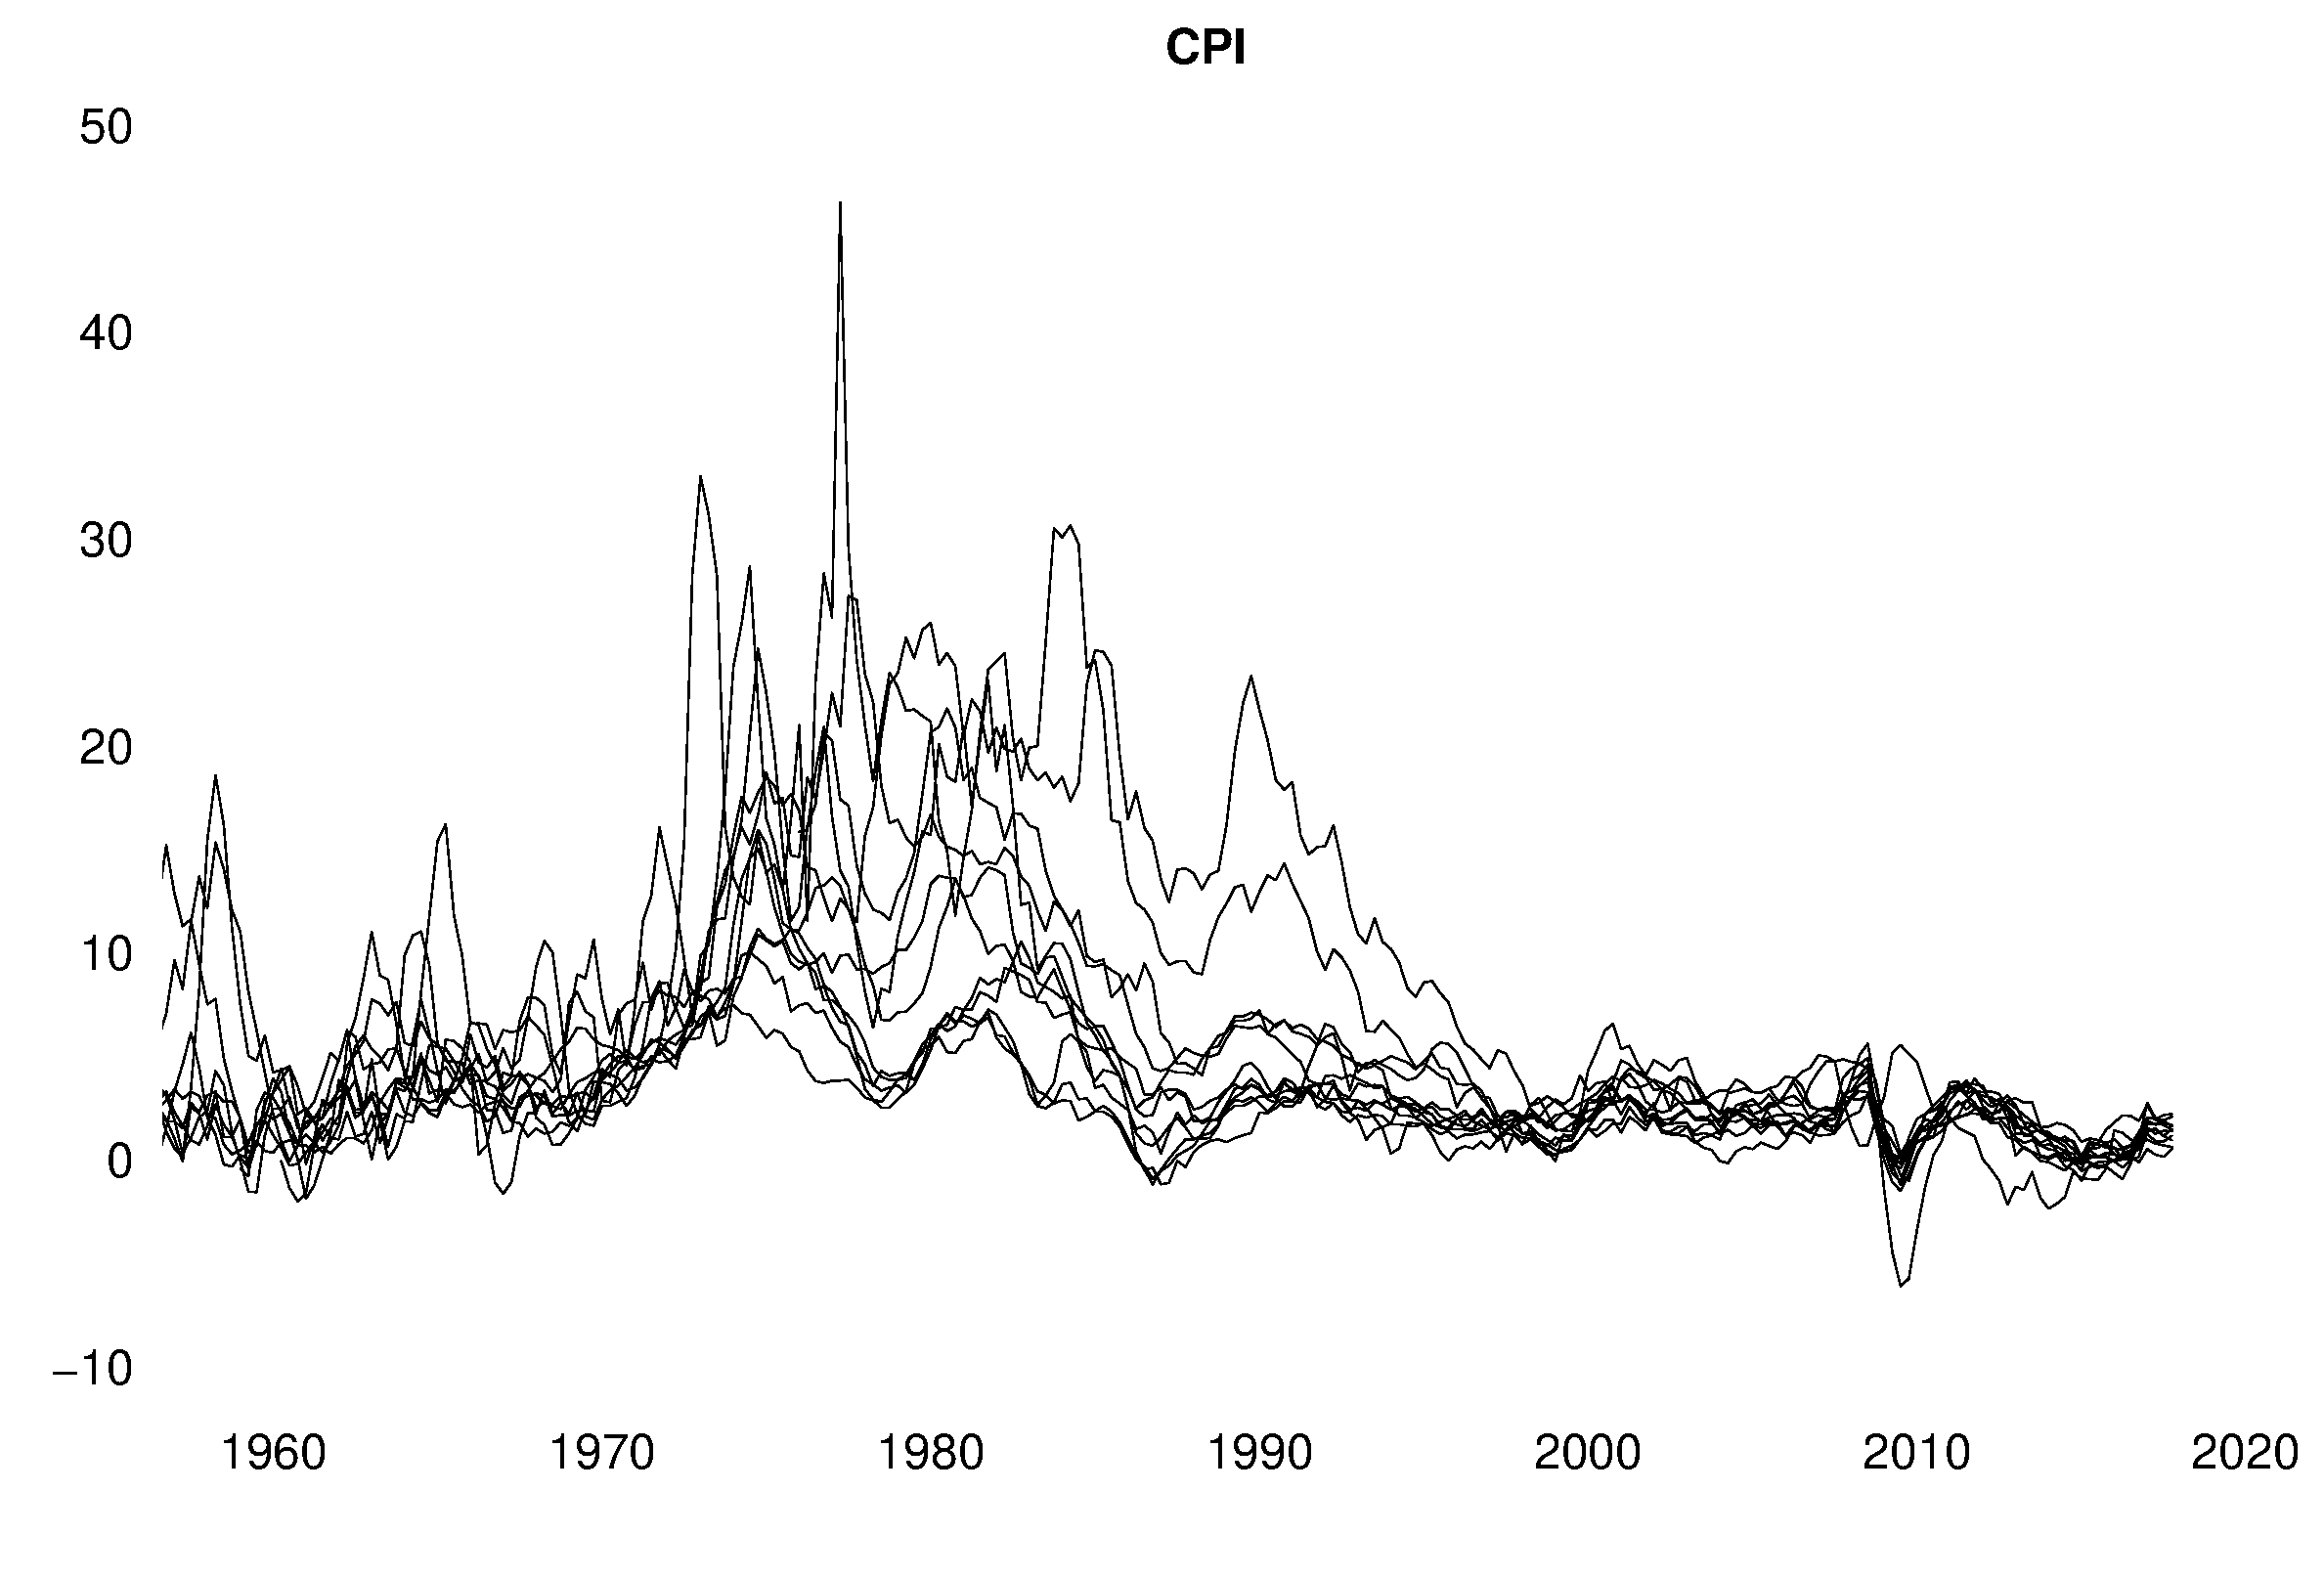
\includegraphics[scale=.29]{cpi.eps}
  \end{figure}
\end{frame}
%--------------------------------------

%--------------------------------------
\begin{frame}
  Deutschmark served as anchor for whole system
  \begin{itemize}
    \item De facto autonomy by Bundesbank
    \item Symmetric system became asymmetric
  \end{itemize}
  \medskip
  Two important implications 
\begin{enumerate}
  \item Bundesbank leadership not popular with other countries
  \item 1991-1992 crisis: breakdown of ERM in 1992
\end{enumerate}
\end{frame}
%--------------------------------------


%--------------------------------------
\begin{frame}
  Eventually three events brought down the ERM
\begin{enumerate}
  \item German Reunification
  \item Denmark rejecting the Maastricht Treaty
  \item French referendum
\end{enumerate}
\end{frame}
%--------------------------------------

%--------------------------------------
\begin{frame}
  \textbf{German reunification} (1991)\\
    High inflation risk due to state of East Germany: Bundesbank increased interest rate to quell risk
    \begin{itemize}
      \item Some countries did not follow due to economic slowdown
      \item Triggered speculative attacks on countries that lost competitiveness
    \end{itemize}
\end{frame}
%--------------------------------------

%--------------------------------------
\begin{frame}
 \textbf{Danish referendum}\\
   First to ratify the Maastricht Treaty
   \begin{itemize}
     \item Danes voted against it; sparked contagion fears     
   \end{itemize}
   \medskip
   \textbf{French referendum}\\
   Similar to Denmark: poll did not look good
   \begin{itemize}
     \item Again, contagion fears
     \item Unrest in exchange market, specifically Italian Lira and British Pound
   \end{itemize}
\end{frame}
%--------------------------------------

%--------------------------------------
\begin{frame}
  \textbf{Black Wednesday}
  \begin{itemize}
    \item 1987: Sterling pegged; prevents fluctuations of more than 6\%
    \item 1990: Joined ERM
    \item 1992: German interest rate, and other ERM turmoil, puts pressure on Sterling
    \begin{itemize}
      \item HMG increased interest rate: spends billions worth of foreign currency to support the Sterling
    \end{itemize}
    \item 1992: Investors keep selling Sterling for foreign currency
  \end{itemize}
  \medskip
  Wednesday 16 Sept: UK leaves ERM
  \begin{itemize}
    \item George Soros might 1B\$ profit on this
  \end{itemize}
\end{frame}
%--------------------------------------

%--------------------------------------
\begin{frame}
  \begin{figure}
    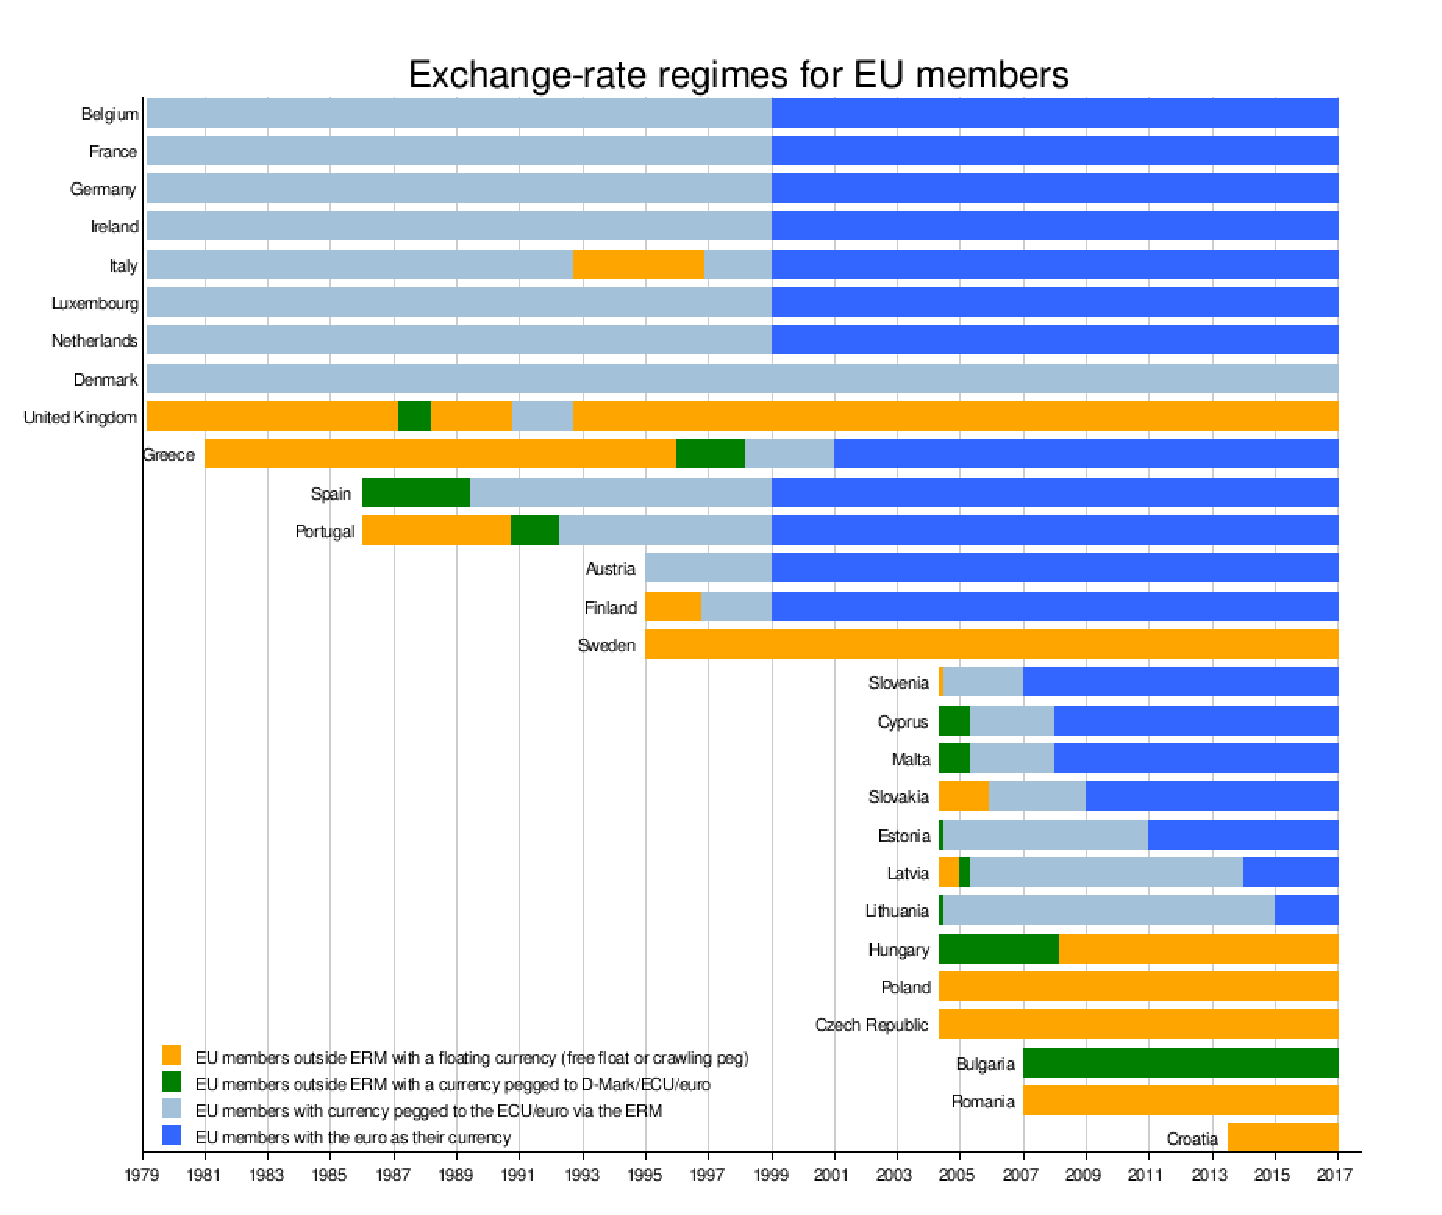
\includegraphics[scale=.4]{erm.eps}
  \end{figure}
\end{frame}
%--------------------------------------

%--------------------------------------
\begin{frame}
  EMU is based on three main principles
  \begin{enumerate}
    \item Provide price stability
    \item Central bank independence
    \item Fiscal discipline  
\end{enumerate}
\end{frame}
%--------------------------------------

%--------------------------------------
\begin{frame}
  \textbf{Price stability}\\
  Surprisingly, treaty itself does not give definition: Eurosystem states following
  \begin{quote}
    ..the year-on-year increase in the Harmonised Index of Consumer Prices for the Eurozone of close to but below 2 per cent. Price stability is to be maintained over the medium term .
  \end{quote}
   \medskip
   Most central banks keep inflation 1.5-2\% over 2-3y
   \begin{itemize}
     \item Short run: monetary policy affects inflation, growth, and unemployment
     \item Long run: monetary policy only impacts inflation     
   \end{itemize}
\end{frame}
%--------------------------------------

%--------------------------------------
\begin{frame}
  \textbf{Central bank independence} entails that central bank should be able to work without outside interference
  \begin{itemize}
    \item Main aim central bank: price stability
    \item Other (government) don't mind higher inflation rates 
  \end{itemize}  
\end{frame}
%--------------------------------------

%--------------------------------------
\begin{frame}
  \textbf{Fiscal discipline} required to create conditions under which central bank can operate effectively
  \begin{itemize}
    \item Government borrowing could lead to onset financial crisis (at large enough deficit)
    \item Government could spend now, to create goodwill with the population, and tax later after the elections (or never)  
  \end{itemize}
  \medskip
   \textbf{Moral hazard} risk: in monetary union the government could be waiting for fiscal transfers
   \begin{itemize}
     \item Maastricht Treaty prohibits bailouts 
   \end{itemize}    
\end{frame}
%--------------------------------------


%--------------------------------------
\begin{frame} 
  \textbf{EMU and OCA}\\
  \medskip
  EMU not based on OCA theory criteria  
  \begin{itemize}
    \item European leaders decided to use another set of conditions
  \end{itemize}
  \medskip
  Any EU member can join the euro
\begin{itemize}
  \item After they have shown to behave according to Maastricht Treat guiding principles
  \item From 2020 new member states are obliged to join the euro
\end{itemize}
\end{frame}
%--------------------------------------

%--------------------------------------
\begin{frame}
 EMU entry conditions cover five areas
\begin{enumerate}
  \item Inflation
  \item Long-term nominal interest rate
  \item Exchange Rate Mechanism (ERM) membership
  \item Budget deficit
  \item Public debt
\end{enumerate}
\end{frame}
%--------------------------------------

%--------------------------------------
\begin{frame}
  \textbf{Inflation}
  \begin{quote}
    The inflation rate should not exceed the average of the three lowest inflation rates achieved by the EU member state by 1.5 percentage points 
  \end{quote}
    \textbf{Long-run interest rate}
    \begin{quote}
      The long-term interest rate should not exceed by more than 2 percentage points the average observed rate of the three lowest inflation rate countries
    \end{quote}
  \begin{align}
    i \approx r + \pi^e
  \end{align}
  \medskip
  Countries can squeeze prices temporarily: not in long run  
\end{frame}
%--------------------------------------

%--------------------------------------
\begin{frame} 
  \textbf{ERM membership}
  \begin{quote}
    Countries should have taken part in the ERM at least two years without having to devalue its currency 
  \end{quote}  
  \textbf{Budget deficit}
  \begin{quote}
    Budget deficit should not exceed 3 per cent of GDP
  \end{quote}
   \medskip
   German signature: deficit should correspond to public investments           
\end{frame}
%--------------------------------------

%--------------------------------------
\begin{frame}
  \textbf{Public debt} 
  \begin{quote}
    Public debt should not exceed 60\% of GDP
  \end{quote}
  Particular threshold since this was the average level when the treaty was negotiated in 1991
  \begin{itemize}
    \item Actually it is 60\% "or moving in that direction"
    \item Belgium had public debt that exceeded 60\%
  \end{itemize}
  \medskip
  Deficits can be altered by shifting around public spending and tax revenues
\end{frame}
%--------------------------------------

%--------------------------------------
\begin{frame}
  \textbf{Monetary vs. fiscal policy}\\
  \medskip
  Joining EMU, countries give up autonomy over monetary policy
  \begin{itemize}
    \item Set by ECB
  \end{itemize}
  \medskip
  Retain autonomy over fiscal policy
  \begin{itemize}
    \item Within limits of Maastricht Treaty
  \end{itemize}
  \medskip
  Fiscal policy only instrument for government to deal with asymmetric shocks
\end{frame}
%--------------------------------------

%--------------------------------------
\begin{frame}
  Fiscal policy in most cases not good alternative to monetary policy
\begin{enumerate}
  \item Budget needs to be balanced
  \begin{itemize}
    \item Government wants to increase private spending by cutting taxes
    \item Will create budget deficit; needs to be accounted for: government borrows
    \item Borrowing leads debt; needs to be paid off: future tax increase
  \end{itemize}
  \medskip
  \item Slow to implement
  \begin{itemize}
    \item Establishing budget is a long political process
  \end{itemize}
\end{enumerate}
\end{frame}
%--------------------------------------

%--------------------------------------
\begin{frame}
 Nonetheless, counter-cyclical fiscal policies can be effective
  \begin{itemize}
    \item Government can borrow relatively easy compared to households/firms
    \item In CU country hit by shock could borrow money from unaffected countries
  \end{itemize}
  \medskip
  Fiscal policy is counter-cyclical; when economy slows down
  \begin{itemize}
    \item Tax revenues decline
    \item Unemployment benefits will increase
  \end{itemize}  
  \medskip
  Therefore fiscal policy will automatically be expansionary: known as \textbf{automatic stabilizers}  
\end{frame}
%--------------------------------------

%--------------------------------------
\begin{frame}
  \begin{figure}
    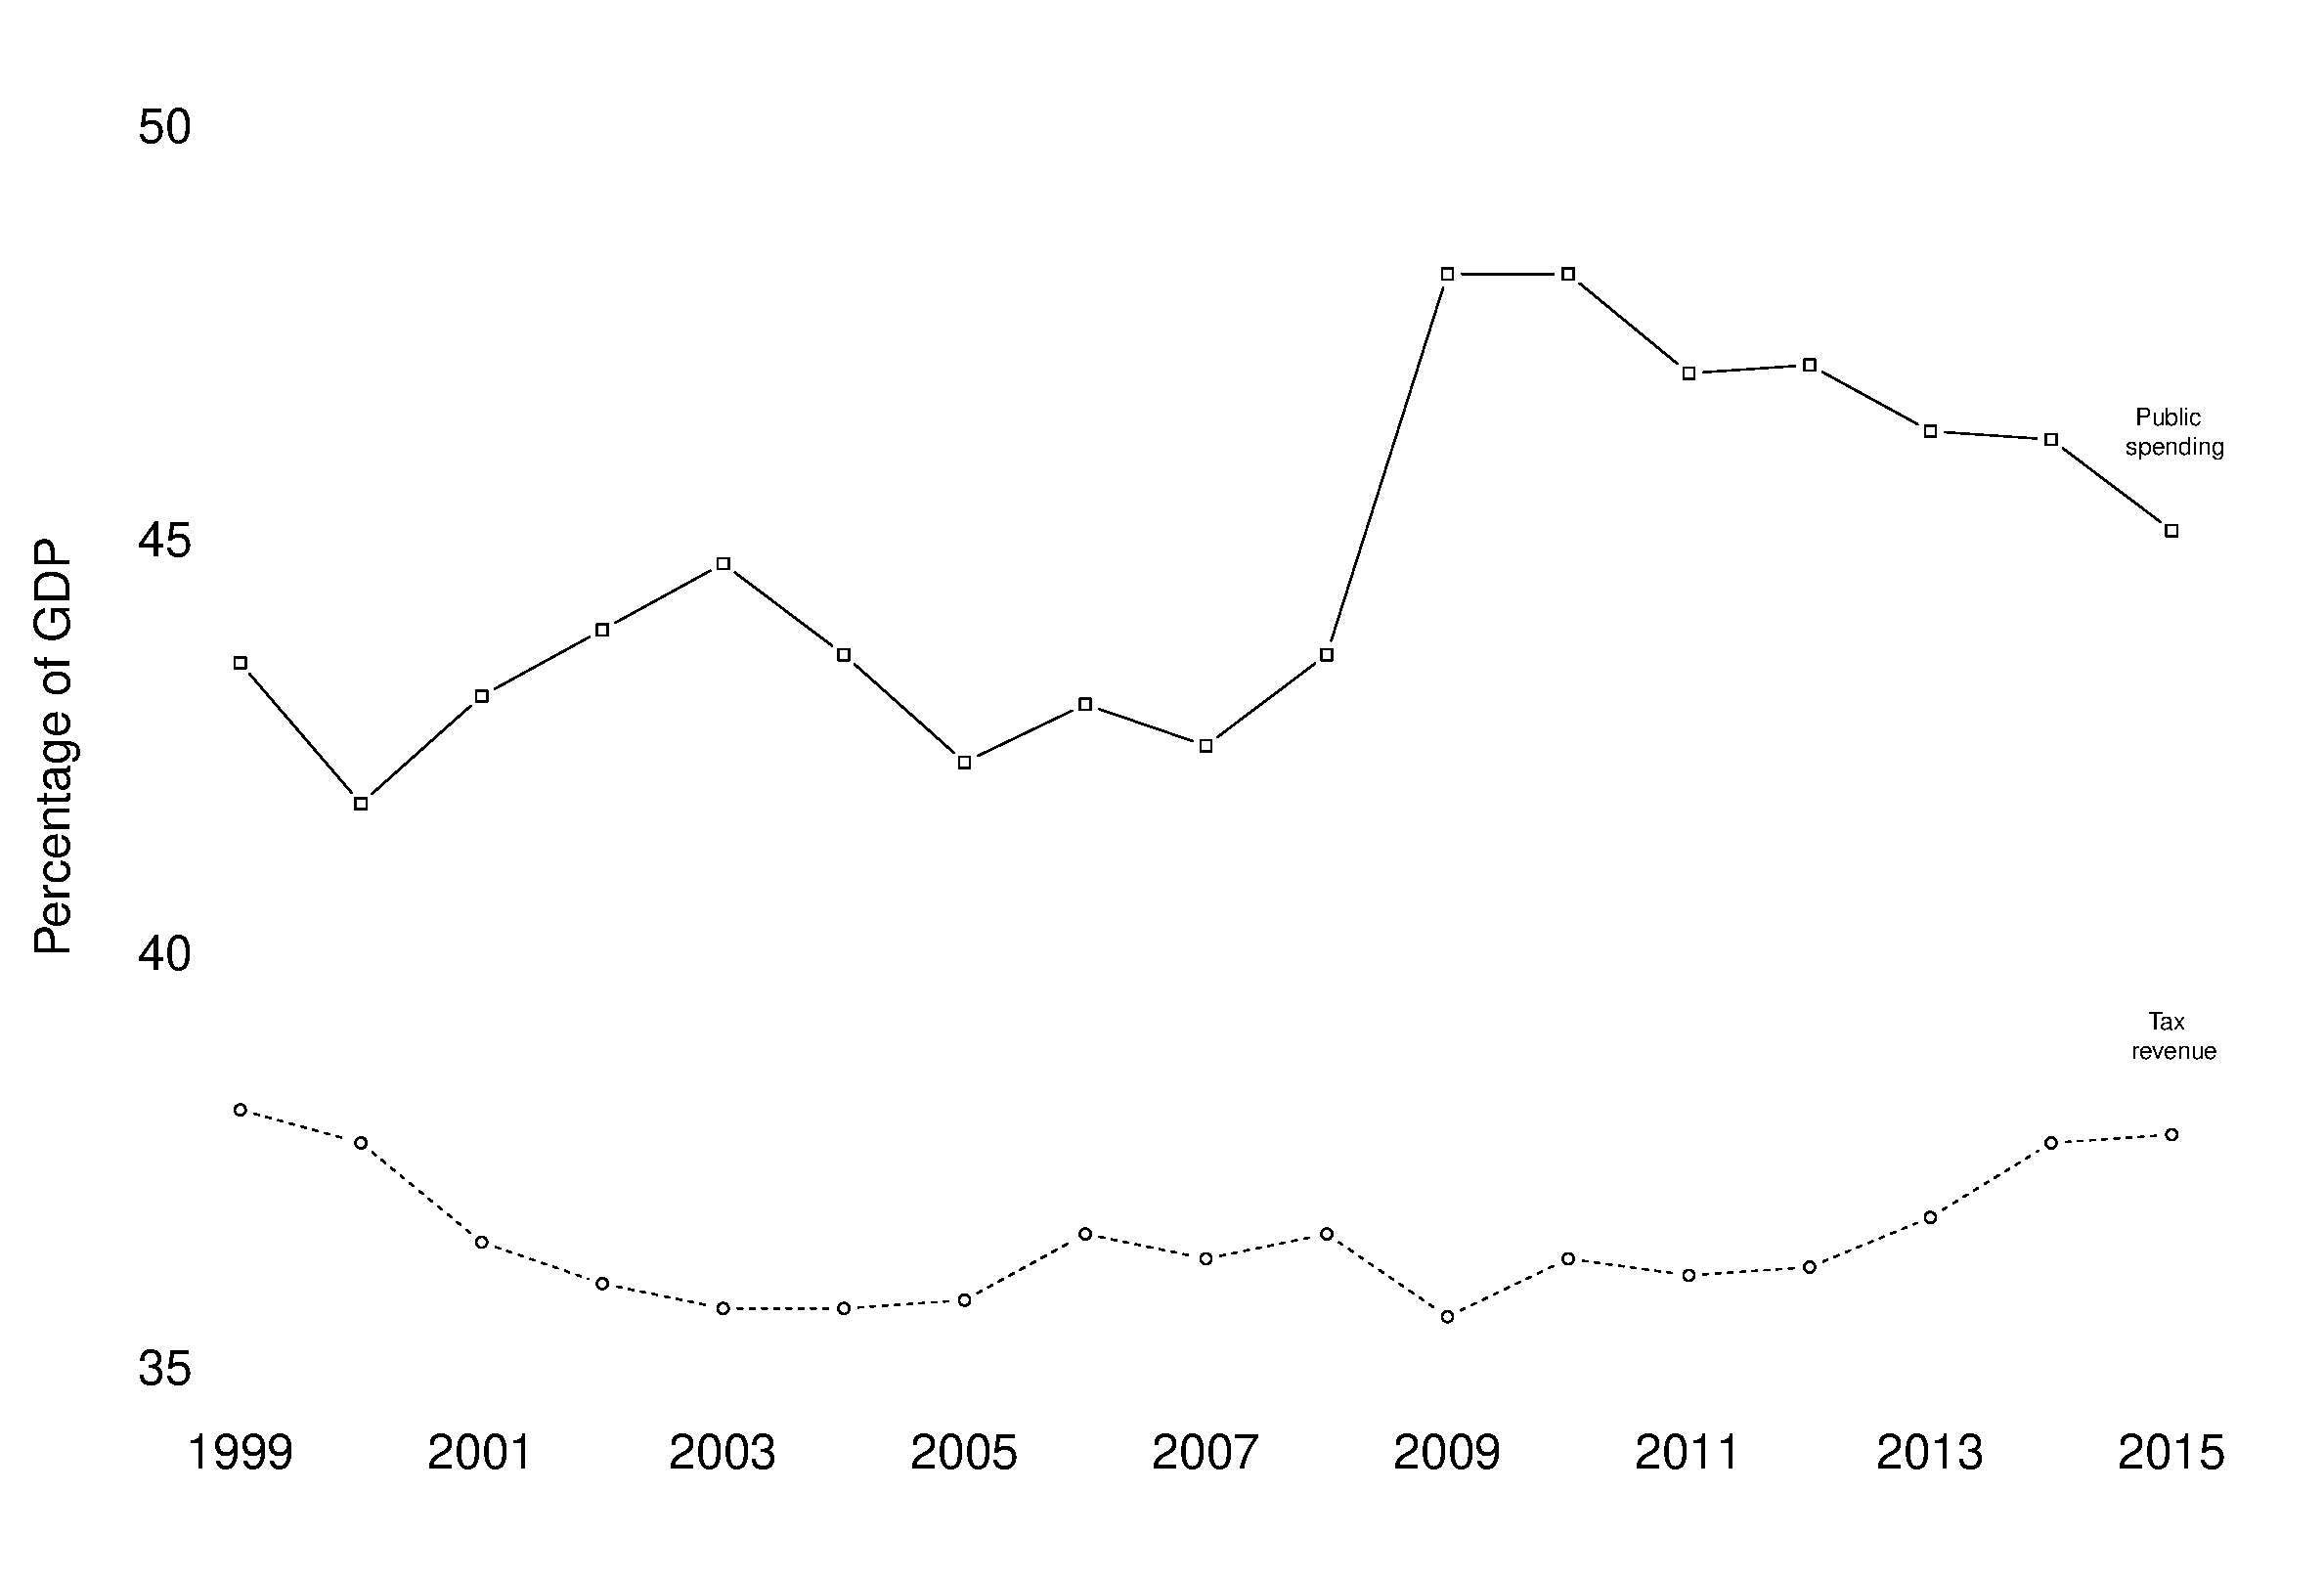
\includegraphics[scale=.3]{automatic_stabilisers.eps}
  \end{figure}
\end{frame}
%--------------------------------------

%--------------------------------------
\begin{frame}
 Automatic stablisers help dampen impact of fluctuations in business cycle
  \begin{itemize}
    \item Discretionary policy is when government takes active action
  \end{itemize}
  \medskip
  Budget figures might obscure government actions  
\begin{enumerate}
  \item Discretionary policy action: budget can improve due to spending cuts or increased taxes
  \item Automatic stabilizers: budget improves due to the fact that the economy is in a boom state
\end{enumerate}
\end{frame}
%--------------------------------------

%--------------------------------------
\begin{frame}
  Use \textbf{cyclically-adjusted budget balance} to disentangle
  \begin{enumerate}
    \item Discretionary policy
    \item Automatic stabilisers
  \end{enumerate}
  \medskip
  Cyclically-adjusted budget balance relies on \textbf{output gap} to measure performance of economy
  \begin{itemize}
    \item Relative to its potential output
  \end{itemize}
\begin{align}
  \tilde{y}=y-y^*
\end{align}
$y^*$ is potential output\\
Difference between the measured budget balance and the cyclically-adjusted budget balance is the work of the automatic stabilizers
\end{frame}
%--------------------------------------

%--------------------------------------
\begin{frame}
  \begin{figure}
    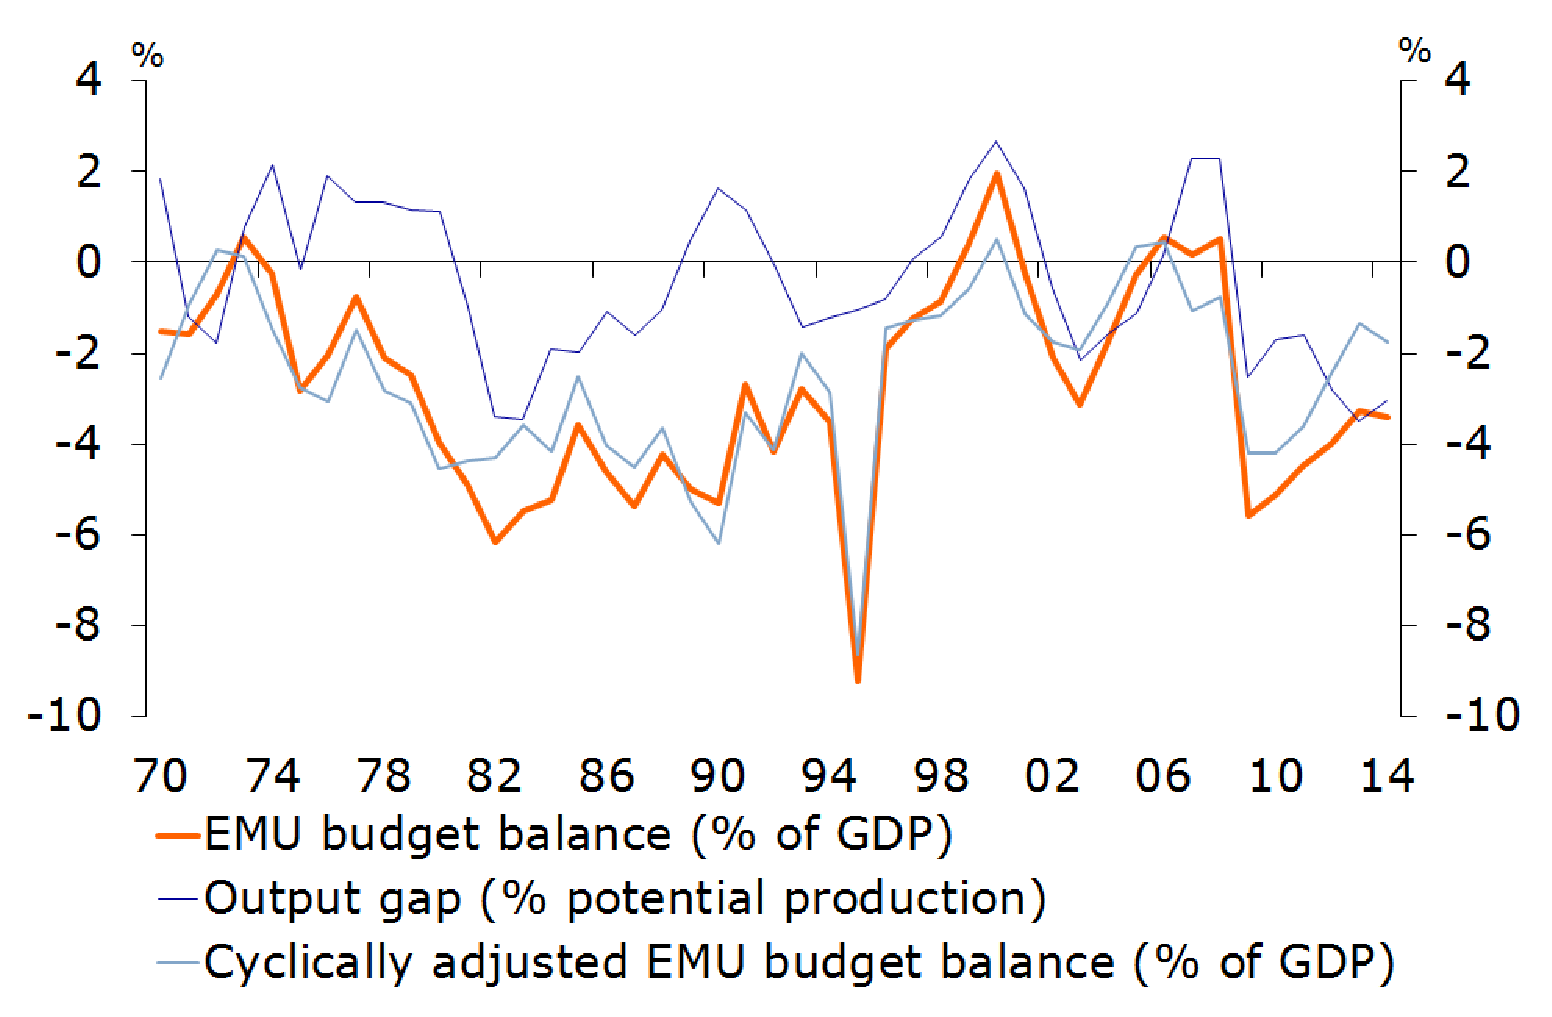
\includegraphics[scale=.4]{nl_budget.eps}
  \end{figure}
\end{frame}
%--------------------------------------


%--------------------------------------
\begin{frame}  
  Why should EU member states coordinate fiscal policy?
  \begin{itemize}
    \item Fiscal policy has spillover effects generating externalities
    \item e.g. business cycles are transmitted via imports/exports
  \end{itemize}
  \medskip
  Makes sense to coordinate policy measures.  
\end{frame}
%--------------------------------------

%--------------------------------------
\begin{frame} 
 Recall EMU entry conditions which included
\begin{itemize}
  \item Budget deficit $\leq$ 3\% of GDP
  \item Public debt $\leq$ 60\% of GDP
\end{itemize}
\medskip
Rules once being a member?
\end{frame}
%--------------------------------------

%--------------------------------------
\begin{frame}
  \textbf{Fiscal discipline} is important pillar of Maastricht Treaty
  \medskip
\begin{itemize}
  \item Stability and Growth Pact (SGP)
  \medskip
  \item Excessive Deficit Procedure (EDP)
  \begin{itemize}
    \item EDP is part of the SGP (currently 11 of 28 member states are subject to an EDP)
  \end{itemize}  
\end{itemize}
\end{frame}
%--------------------------------------

%--------------------------------------
\begin{frame}
  \begin{figure}
    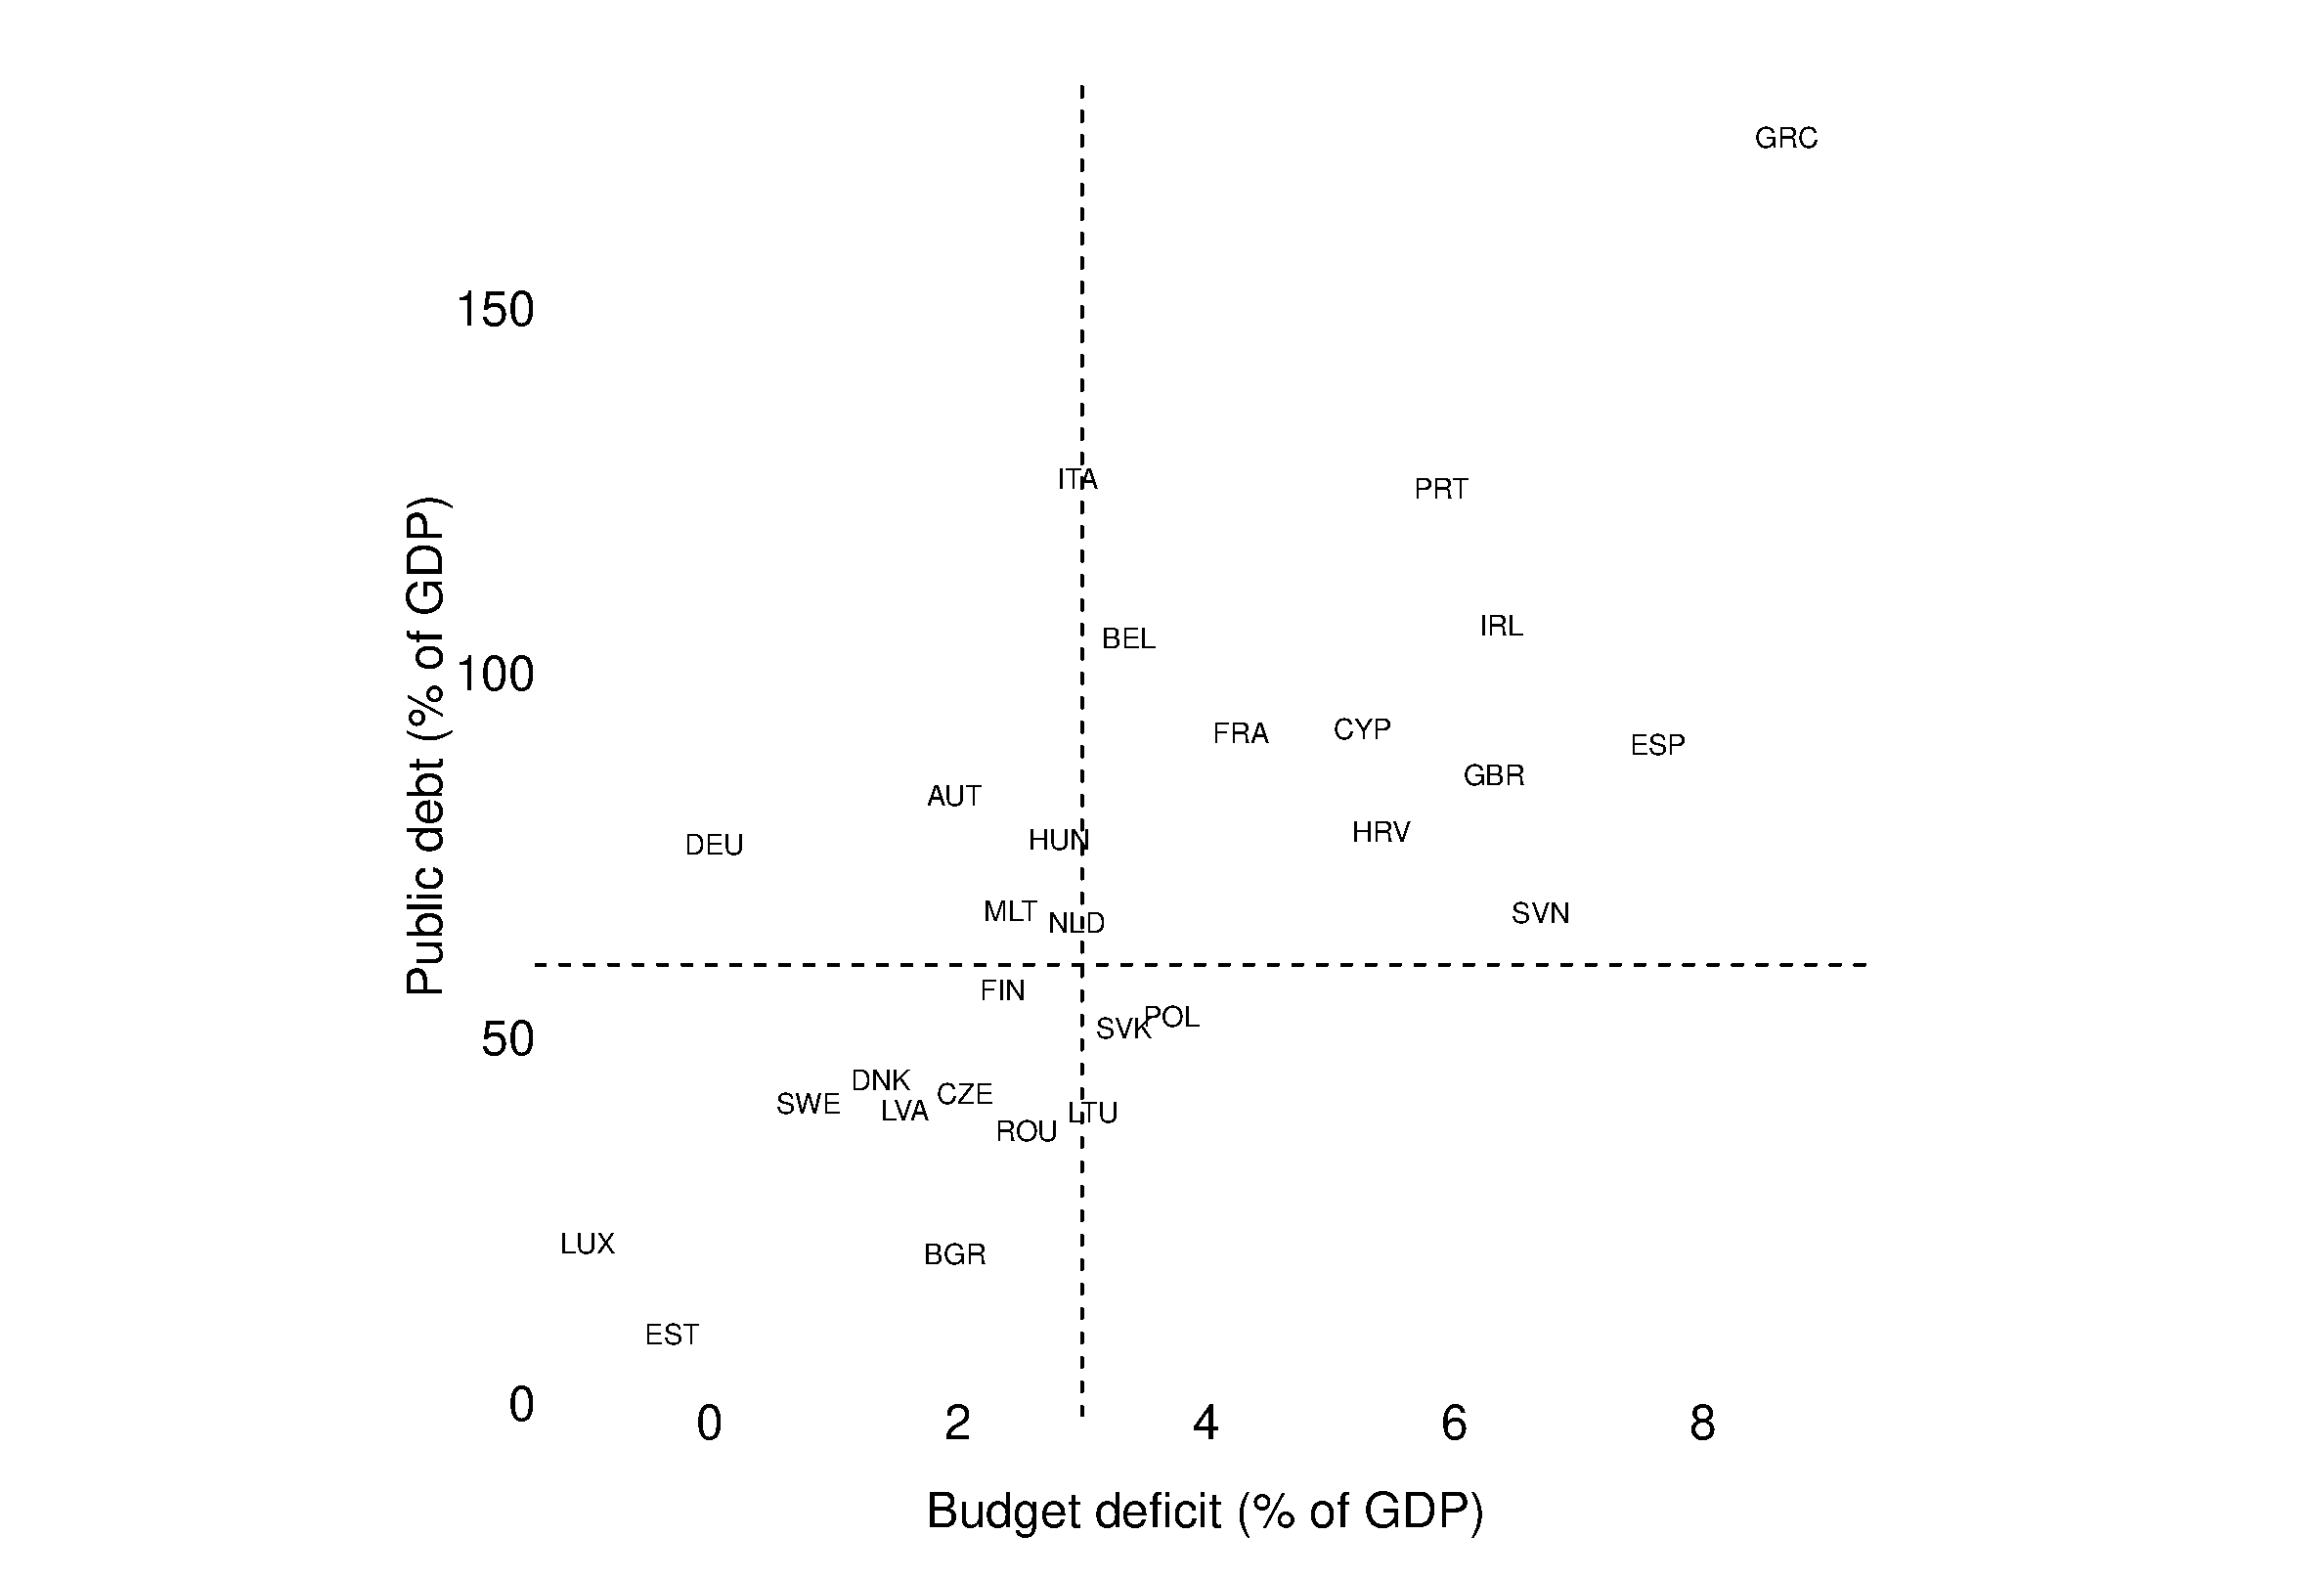
\includegraphics[scale=.3]{fiscal_compliance.eps}
  \end{figure}
\end{frame}
%--------------------------------------

%--------------------------------------
\begin{frame}
  \textbf{Stability and Growth Pact} (1997)\\
  Aim to improve coordination and monitoring of fiscal and other economic policies of the member state
  \begin{itemize}
    \item Enforce deficit and debt limits, as established by Maastricht Treaty
  \end{itemize}
  \medskip
  Main objectives are to ensure that member countries
  \begin{itemize}
    \item Pursue sound public finances
    \item Coordinate fiscal policies
  \end{itemize}
\end{frame}
%--------------------------------------

%--------------------------------------
\begin{frame}
  SGP has evolved over time along with EU's economic governance rules
\begin{itemize}
  \item 1998: Preventive rules of SGP enter into force
  \item 1999: Corrective rules of SGP enter into force
  \item 2005: SGP amendment
  \begin{enumerate}
    \item Better consideration of national circumstances
    \item More economic rationale to rules
  \end{enumerate}
  \medskip  
  \item 2011: Six Pack 
  \item 2013: Two pack and Fiscal Compact
  \item 2014: Review of SGP
  \item 2015: SGP flexibility; European Commission issuing guidance on how rules will be applied
\end{itemize}
\end{frame}
%--------------------------------------

%--------------------------------------
\begin{frame}
  SGP based on three main elements
\begin{enumerate}
  \item Prevention (1998)
  \item Correction (1999)
  \item Enforcement (1999)
\end{enumerate}
\end{frame}
%--------------------------------------

%--------------------------------------
\begin{frame}
  \textbf{Prevention}\\
    Each EU member state is set a budgetary target in order to bind the government to their commitment towards sound fiscal policy and coordination
    \begin{itemize}
      \item Medium-Term Budgetary Objective (MTO), updated every three years
      \item Budget deficit is defined in structural terms: Takes into account the business cycle and filters out one-off or temporary measures
    \end{itemize}
    Member state has to provide an annual budget outlining how to reach the targets, which is assessed by the European Commission and the EU governments
    \begin{itemize}
      \item Rules apply to both Eurozone countries and all other EU member states.  
    \end{itemize}
\end{frame}
%--------------------------------------

%--------------------------------------
\begin{frame}
  \textbf{Correction}\\
  Excessive Debt Procedure (EDP) enters into play when there is excessive debt 
  \begin{itemize}
    \item Ensures correction excessive budget deficits $>3$\% of GDP or public debt levels $>60$\%
    \item Debt levels are excessive when it exceeds 60\% of GDP and does not diminish at an adequate rate of 5\% per year on average over the last three years
  \end{itemize}
  \medskip
  EDP is step-by-step procedure coordinated by European Commission using data from Eurostat
\end{frame}
%--------------------------------------

%--------------------------------------
\begin{frame}
  \textbf{Excessive Debt Procedure}
  \begin{enumerate}
    \item European Commission reports whether to open EDP
    \item European Council decides if excessive debt exists; if so, open EDP
    \item Member state is given recommendations, deadlines, and targets (sometimes sanctions)
    \item 3-6 months for member state to comply with recommendations
    \item European Commission assesses if action taken is sufficient: informs European Council
    \begin{enumerate}[i]
      \item Sufficient $\rightarrow$ council takes note
      \begin{itemize}
        \item European Commission proposes EDP abrogation, Council takes final decision
      \end{itemize}
      \item Targets missed $\rightarrow$ new recommendations; extend deadlines
      \item No effective action $\rightarrow$ new recommendations
      \begin{itemize}
        \item Sanctions if member state is in Eurozone
      \end{itemize}
    \end{enumerate}
  \end{enumerate}
\end{frame}
%--------------------------------------


%--------------------------------------
\begin{frame}
  \textbf{Enforcement}\\
   Sanctions may follow when countries fail to respect the preventive and corrective rules.\\
   Eurozone countries these could be fines
    \begin{itemize}
      \item 0.2\% of GDP, if they fail to abide by either the preventive or the corrective rules
      \item 0.5\% of GDP, if they repeatedly fail to abide by the corrective rules
    \end{itemize}
    \medskip
    For all member states the penalty could be suspension of commitments/payments of the structural and investment funds
    \begin{itemize}
      \item UK is excluded from these penalties
      \item Rules hardly ever enforced on Germany and France
    \end{itemize}    
\end{frame}
%--------------------------------------

%--------------------------------------
\begin{frame}
  \textbf{Six Pack}\\
  Adjustment of economic governance rules following sovereign debt crisis
\begin{enumerate}
  \item Operate public accounting systems that comprehensively cover all areas of income and expenditure
  \item Make the fiscal data publicly available (monthly basis for central and state governments, quarterly for local governments)
  \item Ensure their fiscal planning is based on realistic macroeconomic and budgetary forecasts, using the most up-to-date data
  \item Operate specific fiscal rules to help ensure the overall government budget complies with European rules
  \item Establish a credible, effective medium-term budgetary framework that includes a 3 year fiscal planning horizon
  \item Ensure consistency and coordination of all accounting rules and procedures across all areas of government activity
\end{enumerate}
\end{frame}
%--------------------------------------

%--------------------------------------
\begin{frame}
  Six-pack objective was to 
  \begin{itemize}
  \item Enhance marcoeconomic surveillance
  \item Improve procedures to address public deficits and other macroeconomic imbalances 
  \end{itemize}
  \medskip
  Followed in 2013 by additional rules
  \begin{itemize}
    \item Two Pack: increase in reporting frequency, to enhance surveillance
    \item Fiscal Compact: stricter interpretation of SGP specifically concerning budgetary targets
  \end{itemize}
  \medskip
  Fiscal Compact part of Treaty on Stability, Coordination, and Governance
  \begin{itemize}
    \item Signed by all member states except for Czechia, the United Kingdom, and Croatia
  \end{itemize}
\end{frame}
%--------------------------------------

%--------------------------------------
\begin{frame}
  Expanding the eurozone
  \begin{itemize}
    \item 2004, 10 countries joined the EU; 8 former socialist states
    \item 3/10 have not joined eurozone: Czechia, Hungary, Poland
    \begin{itemize}
      \item Denmark \& Sweden also retain their currency
    \end{itemize}
  \end{itemize}
  \medskip
  Given design of euro and history of new member states one can wonder whether joining the euro
  \begin{enumerate}
    \item Is sensible for these countries?
    \item Beneficial for the eurozone?
  \end{enumerate}
\end{frame}
%--------------------------------------

%--------------------------------------
\begin{frame}
  \begin{figure}
    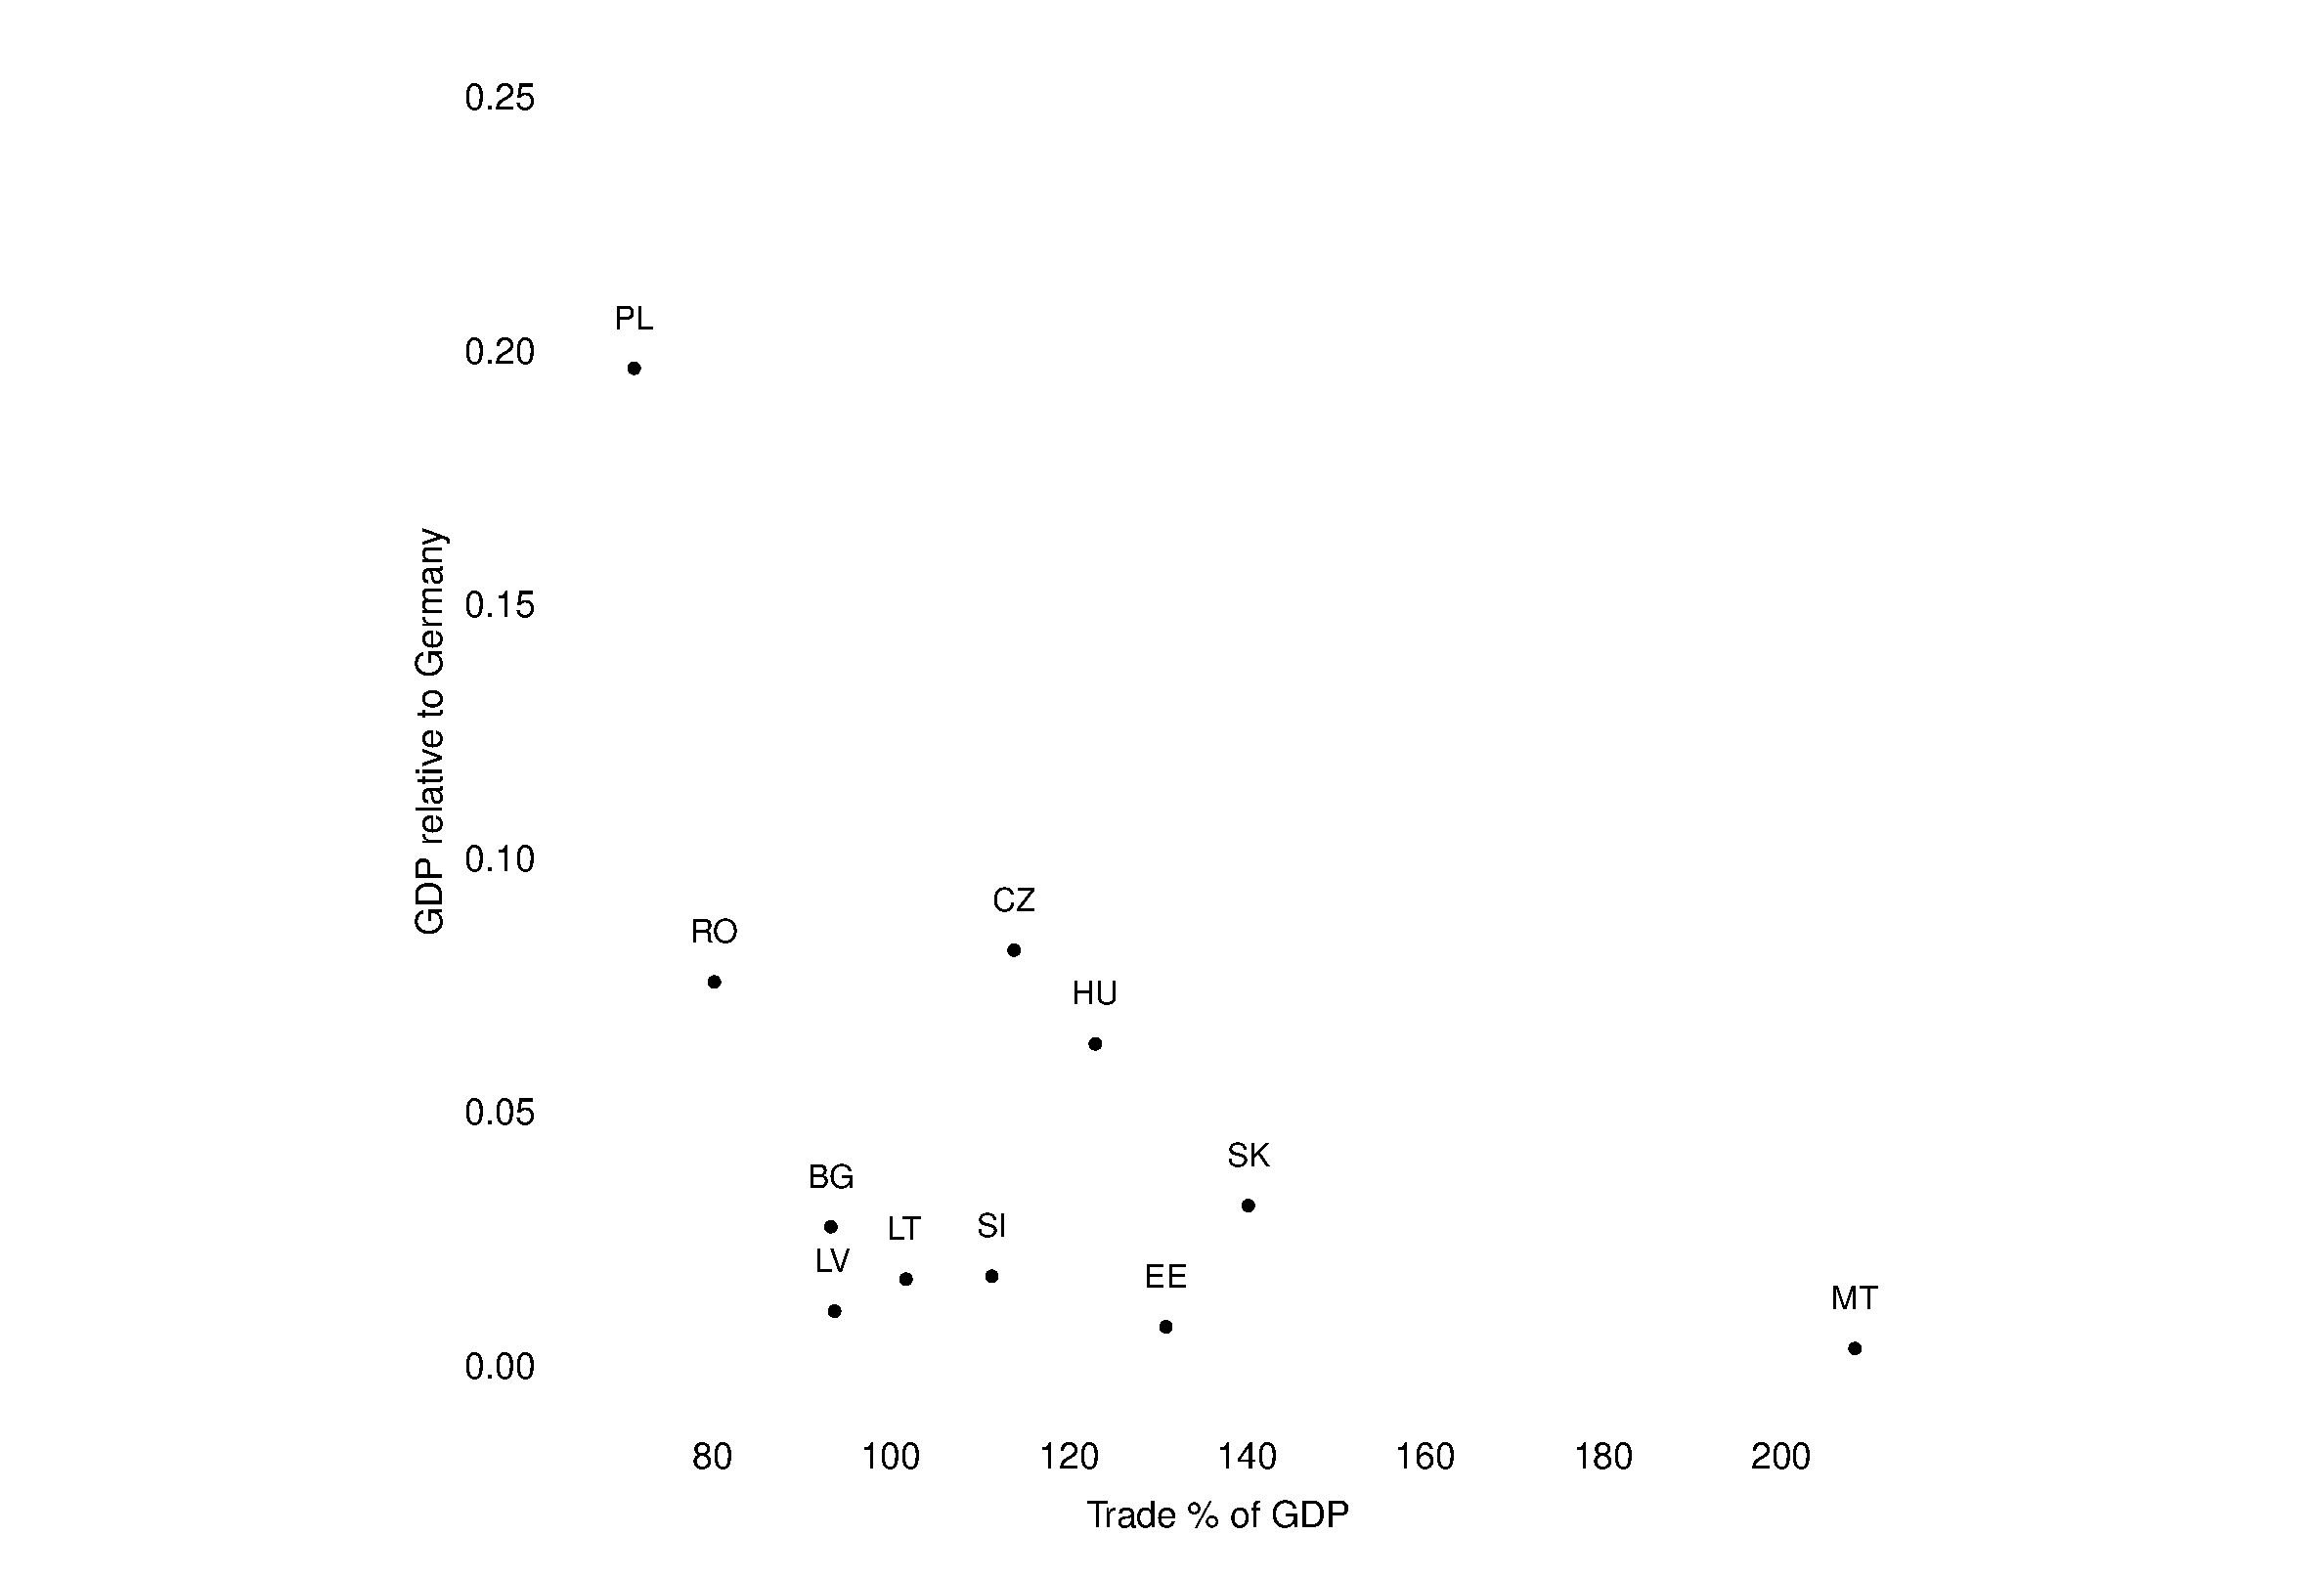
\includegraphics[scale=.3]{trade_new_members.eps}
  \end{figure}
\end{frame}
%--------------------------------------

%--------------------------------------
\begin{frame}
 Joining the euro would make sense given   
\begin{itemize}
  \item Relative small size of economies
  \item Openness to trade
  \item Vulnerability to speculative attacks on their currency
\end{itemize}
\end{frame}
%--------------------------------------

%--------------------------------------
\begin{frame}
  \begin{figure}
    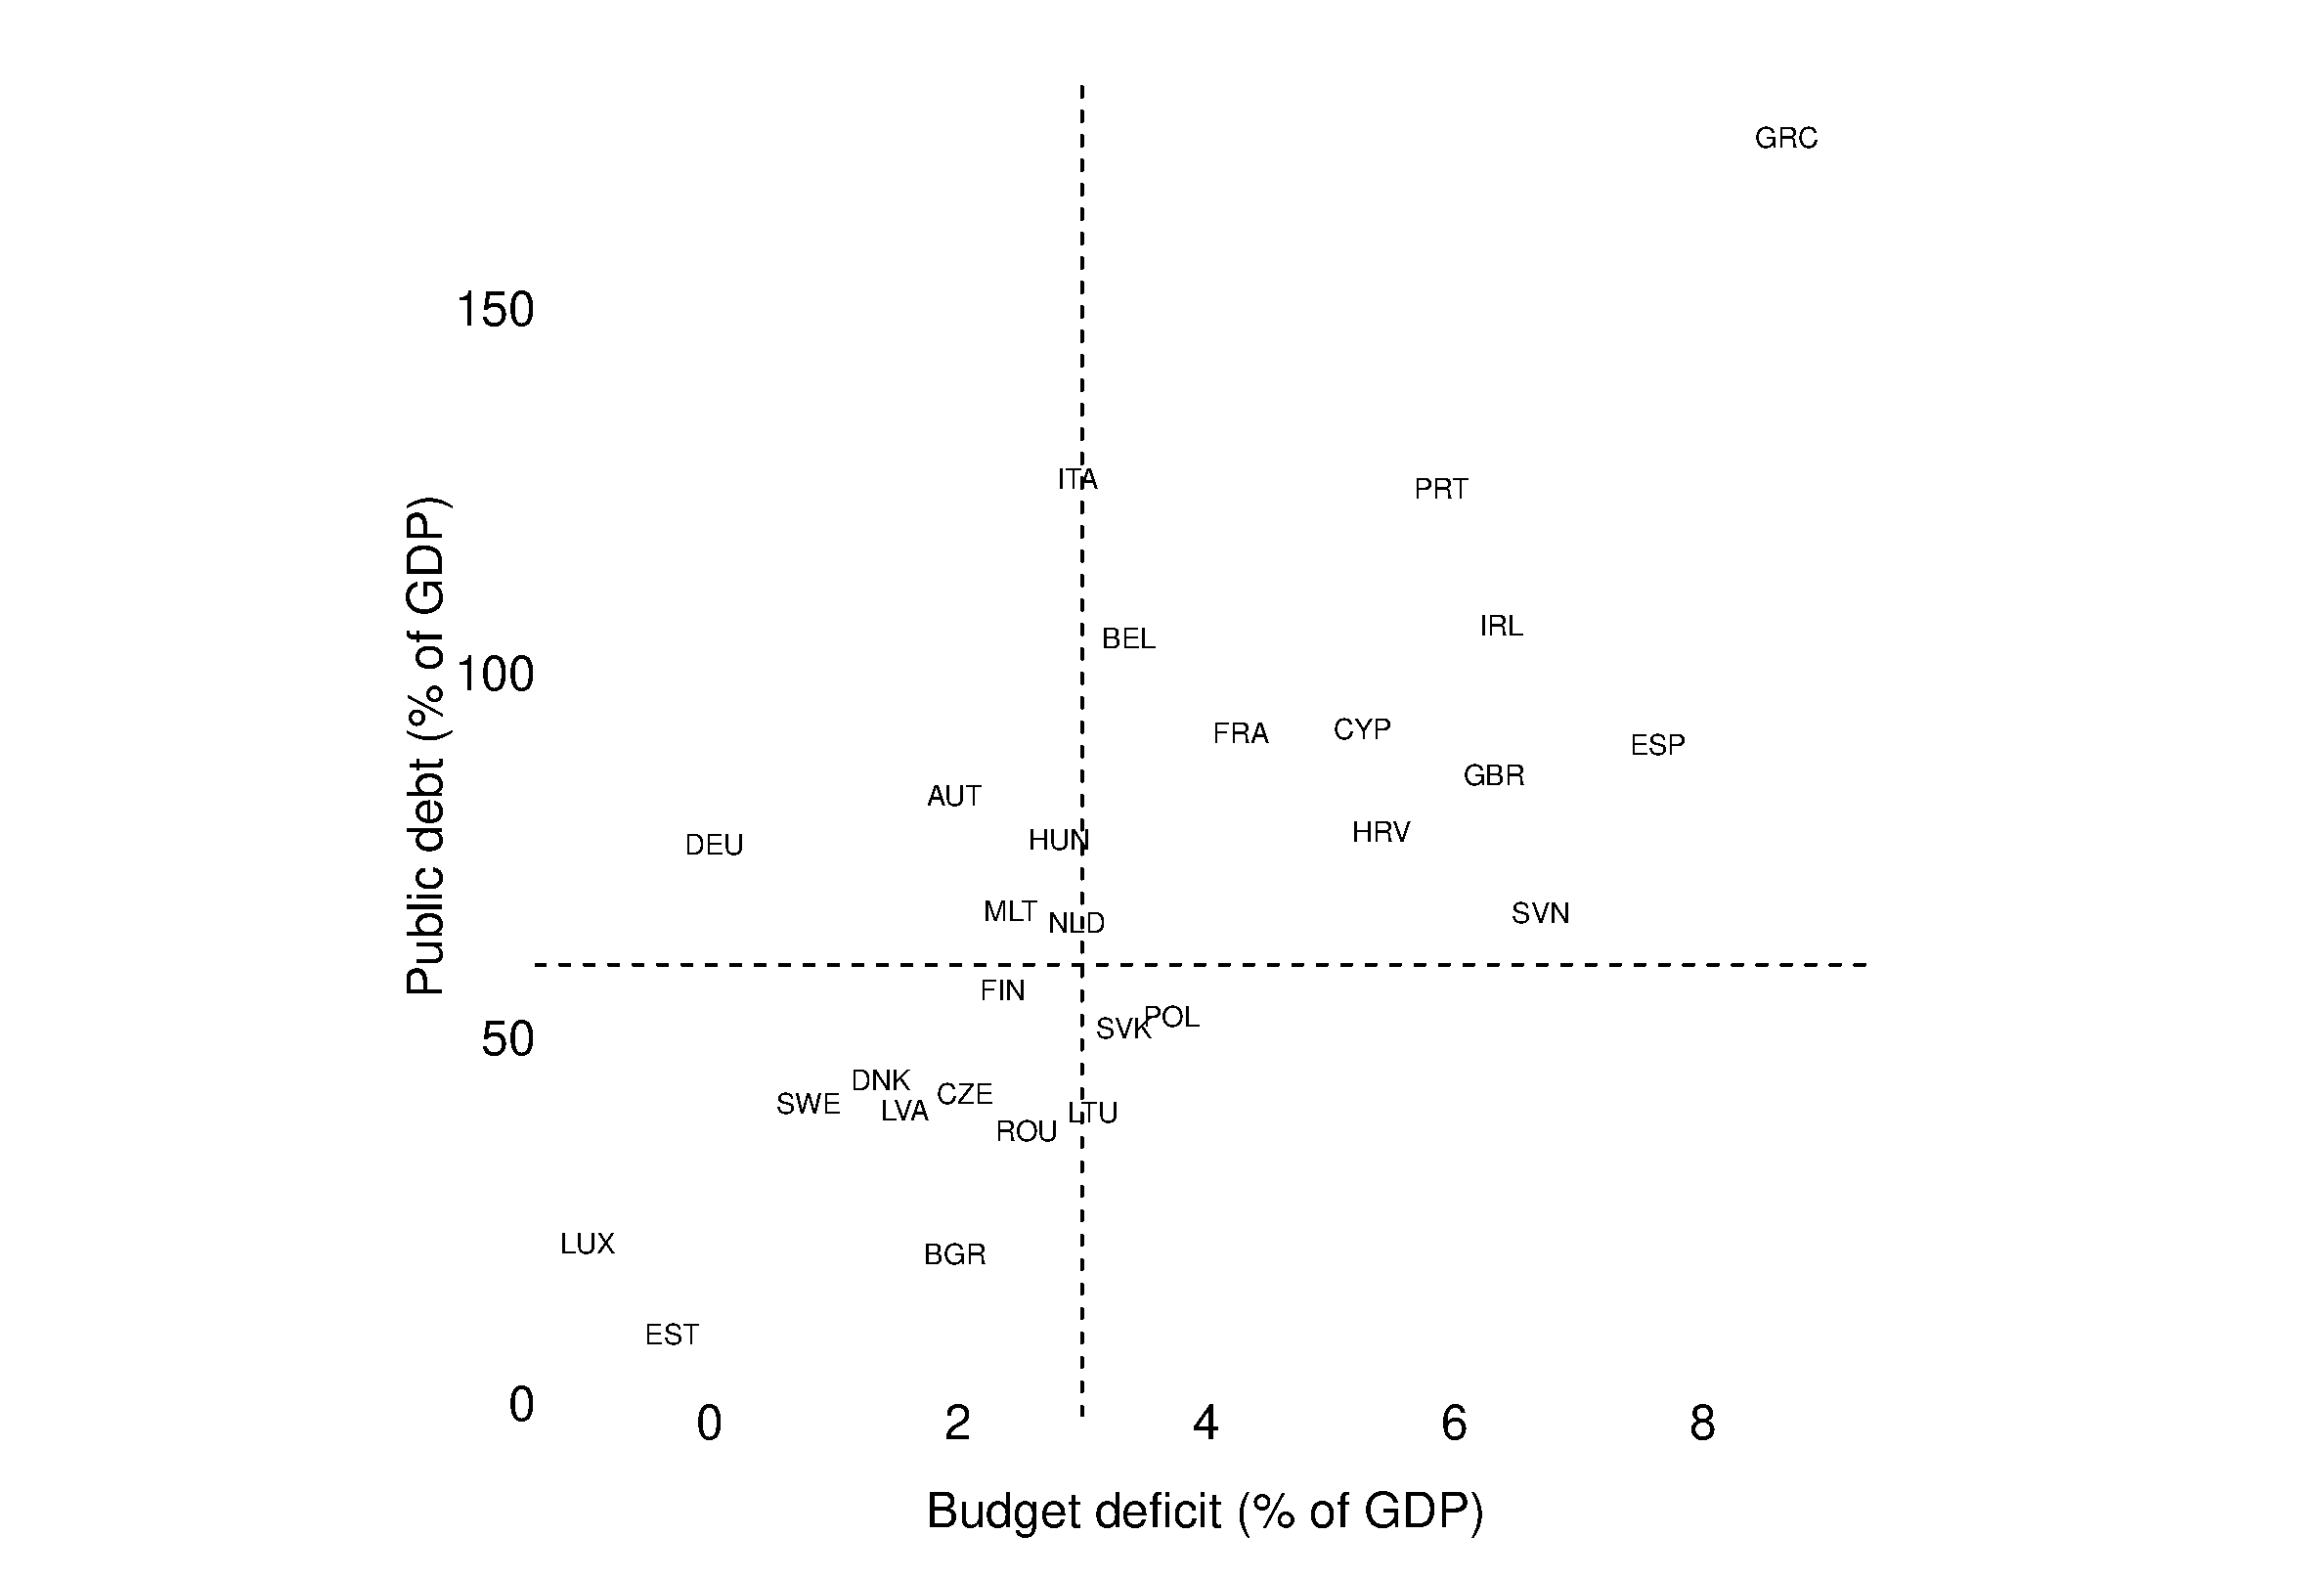
\includegraphics[scale=.3]{fiscal_compliance.eps}
  \end{figure}
\end{frame}
%--------------------------------------

%--------------------------------------
\begin{frame}
  \begin{figure}
    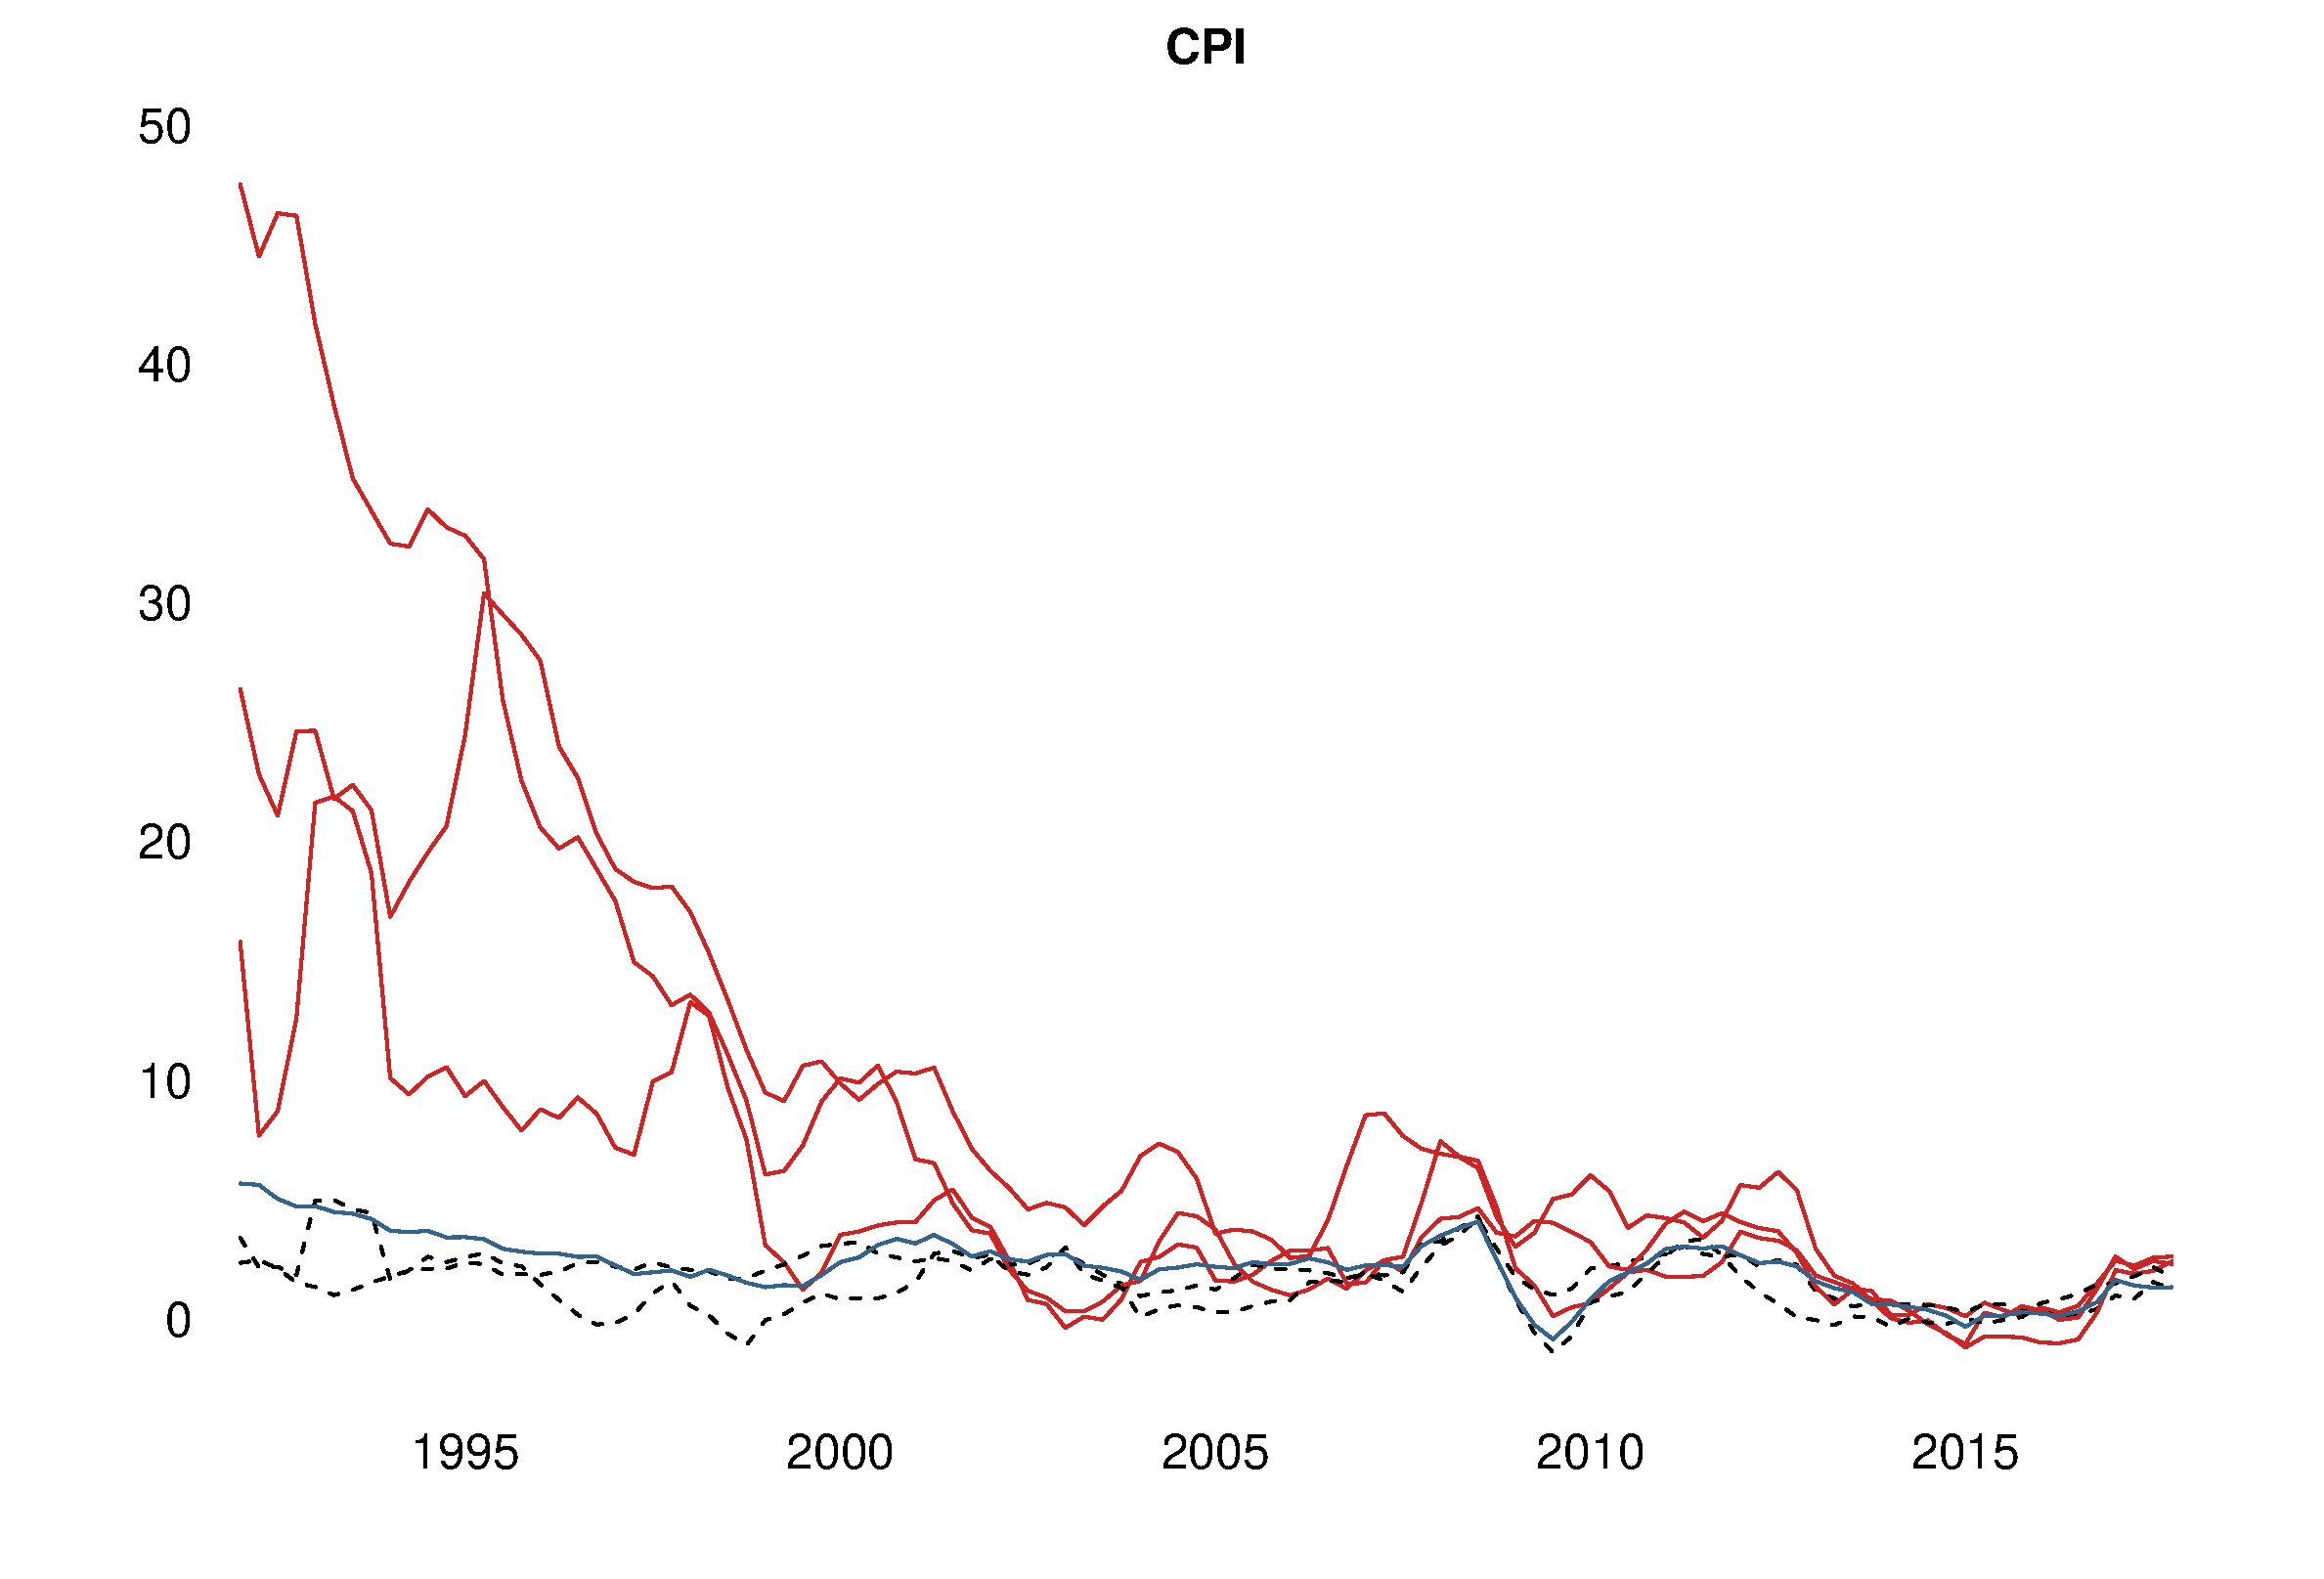
\includegraphics[scale=.3]{inflation_non_eurozone.eps}
  \end{figure}
\end{frame}
%--------------------------------------


%--------------------------------------
\end{document}
